\section{项目背景}

随着智能化控制的进步,工业4.0时代逐渐到来,智能制造与智能家居产业发展迅速,机器人也慢慢走近每家每户。\ 目许多家庭中配备了扫地机器人用来自动清扫地面,让人在每天忙碌的工作后不必再面对扫地的烦恼。\ 智能家庭机器人Jibo能够识别人的情感并与人产生交互,为家庭生活平添了一份乐趣。\ 而在未来,智能家居机器人可能成为家庭的一员,完成更加复杂的任务,辅助人们日常的工作、学习、娱乐,替代人类完成繁杂、琐碎的家务活。\

\begin{figure}[H]
\begin{minipage}[t]{0.5\textwidth}
	\centering
    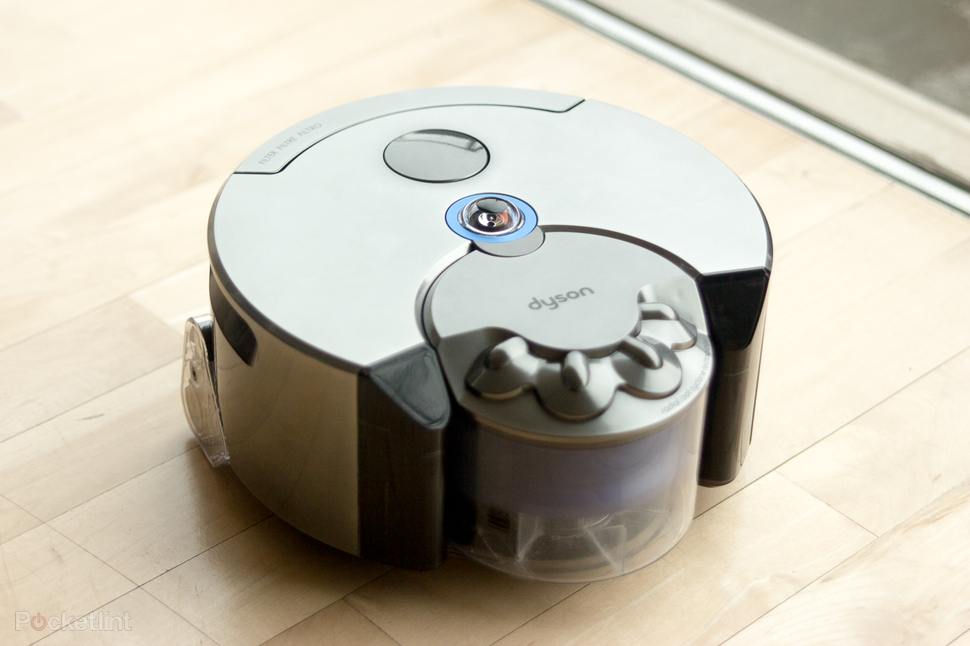
\includegraphics[width = 0.8\textwidth]{pictures/dyson.jpg}
    \caption{Dyson扫地机器人}
    \label{fig:dyson}
\end{minipage}
\begin{minipage}[t]{0.5\textwidth}
	\centering
    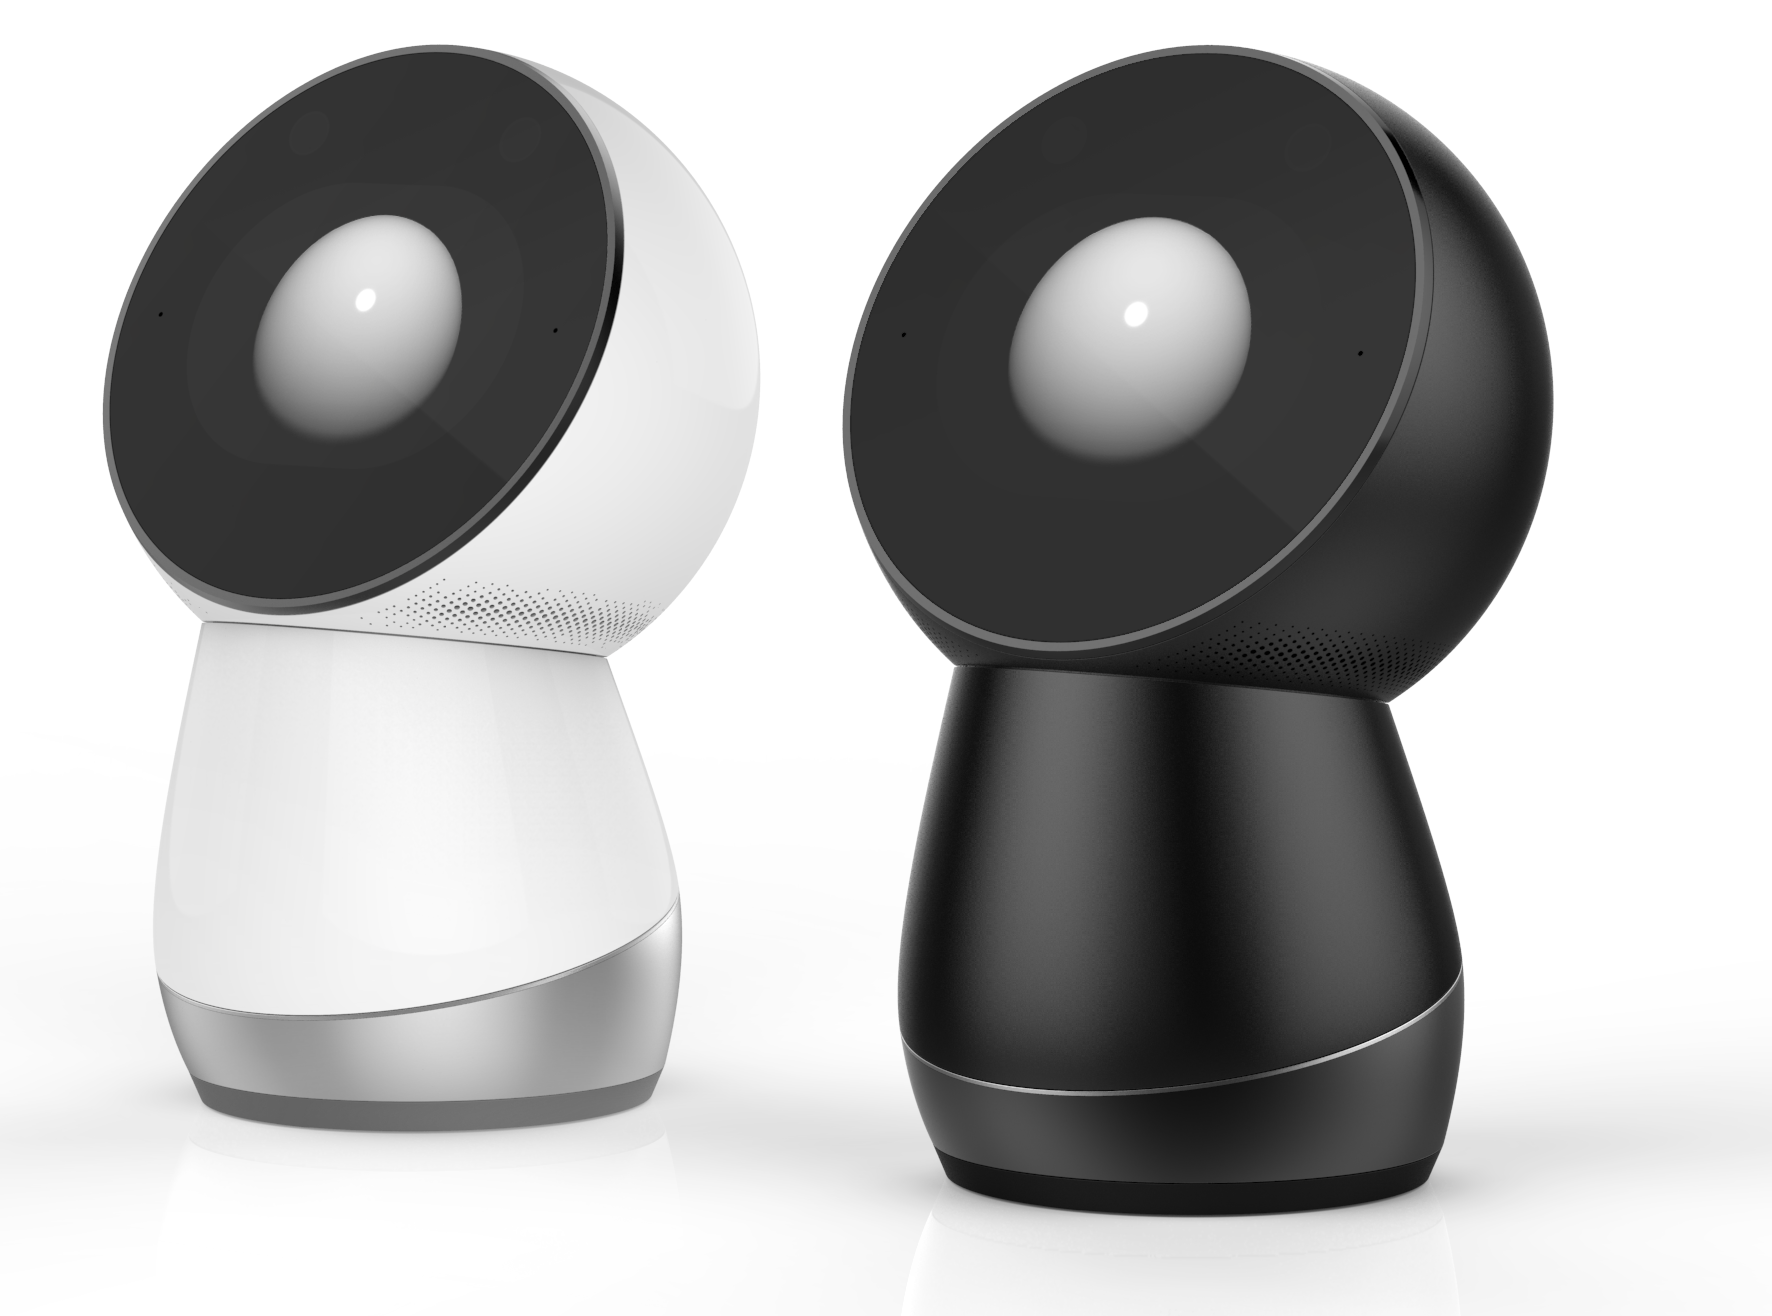
\includegraphics[width = 0.8\textwidth]{pictures/jibo.png}
    \caption{Jibo家庭机器人}
    \label{fig:jibo}
\end{minipage}
\end{figure}

目前,市场上大多数的家庭机器人还都停留在小型的阶段,虽然在软件上已经达到了能感知环境、理解情感、流畅交流的程度,但仍然无法摆脱自身硬件方面的限制,不能帮助完成许多日常生活中看似简单的任务。\ 我们在日常生活中最基本的操作就是拿取物品,而小型的机器人由于体型过小或没有可移动部分,无法做出这些动作,更不可能做出把一个指定的东西送到手边、整理桌上杂乱物品这类更加复杂的动作。\ 另外,目前的智能电器大多只是一个个分立的器件,无法构成一个整体,给人造成了许多的不方便。\ 比如,智能洗衣机在洗完衣服后仍然需要人去晾衣服,智能冰箱也还需要人去开门拿食材。\ 这些“最后一步”的问题也让智能家居的体验大打折扣。\ 

因此,我们希望实现一个可以移动的机械臂,能够在日常的生活场景中自动识别并抓取、放置物体,连接人与物品,连接人与家居。\ 它能从摆放了各种物品的柜子上帮你取下指定的那一个,或者把桌上杂乱的物体排列整齐。\ 基本的物体操纵功能在实际生活中使用十分广泛,我们的机械臂也将胜任日常生活中的大部分任务,能帮人大大减轻负担。\ 

\section{项目创新点}

% 机械臂自动抓取在工业与民用领域都有着广泛的应用。\ 在工业上,由于机械臂工作环境固定,故多采用预先编程、开环控制的方式,不能够适应复杂多变的现实环境。\ 另外,也多采用视觉与机械臂分离的方式,在流水线的一个环节中使用机器视觉进行识别,下一个环节通过机械臂姿态解算来抓取物体,整体的集成度不高。

% 对于更加复杂多变的民用场景,也不乏对于机械臂物体操纵的研究。\ 
在复杂多变的现实场景中,机械臂自动抓取的任务较为困难,但目前已经有一些研究成果。\ 瑞士洛桑联邦理工学院的LASA实验室使用能获取关节角度信息的轻量级机械臂KUKA,经过手动训练,通过外部相机的视觉信息能准确抓取飞行中的物体\cite{kim2014catching}。\ 卡内基梅隆大学NREC部门的ARM-S机器人利用三维传感器获得场景点云并提取识别物体,采用关节反馈来准确获得机械臂的位置\cite{nrec}。\ 这些机械臂都内置了关节反馈,对电机精度也提出了较高的要求,导致机械臂制造成本较高。\ 另外,由于缺少机械臂的末端视觉反馈,机械臂在移动时使用开环控制,难以应对现实场景中突发的变化。

为此,我们提出了一套抓取系统,利用灰度熵与准对室内场景优化的算法来分离物体,使用基于稀疏表示的分类器来识别物体,采用末端视觉反馈来引导机械臂的抓取。这套结合了多种算法的系统能够很好地完成室内环境的物品抓取任务。\ 具体创新点如下。

\subsection{使用末端视觉进行视觉伺服}

我们的机械臂最基础的功能就是抓取物体,而在复杂的室内环境中,通过深度视觉获取到的物体位置信息不够准确,加上机械臂本身的旷量与电机角度的误差,若用开环控制机械臂的移动,很容易导致抓取的不准确,还有可能让机械手触碰到附近的其他物体。\ 

为了解决这一问题,我们在机械手上加装了末端摄像头,使用基于图像的视觉伺服(Image-Based Visual Servoing),构成一个手眼(eye-in-hand)机械臂系统,通过末端视觉获得的物体位置作为反馈,构成机械臂移动的闭环控制,保证物体的准确抓取。\ 

\subsection{物体分辨与识别}

物体识别的一般方法是通过计算两个矩阵的标准化降采样矩阵的点击来判断相似性\cite{aldoma2012point},这样做虽然有一定的效果,但结果的点积值却没有实际意义,对于不同的物体相差非常大,因此难以取合适的阈值,判断的鲁棒性不高。\ 

我们采用了基于稀疏表示的分类器来解决这一问题。首先,我们假设当样本数量足够时,每张该物体的照片都可以近似表示为该物体样本照片的线性叠加。随后,使用稳定$L_1$范数最小化问题估算稀疏解,通过残差来确定识别结果。使用这种方式,算法的鲁棒性有了显著的提升,同时速度和存储空间利用效率上并没有显著的降低。\ 

\subsection{灰度熵分离前后景}

在项目的实践过程中,我们需要一种方法,实时地在以书架为背景的典型场景中,找到所有目标物体的三维坐标。\ 已知的目标查找方法有很多,但鉴于环境的复杂性和图片的质量,已知的算法很难在很短的时间内完成标记目标的任务。\ 

我们针对书架场景的特点提出了基于熵过滤的目标查找算法。\ 首先使用灰度熵的方法过滤背景,但对于纯色物体与书架边框区域会产生误判。\ 作为弥补,我们又提出了目标纯色快提取方法和线段检测方法,分别查找纯色物体和过滤书架框架。\ 利用过滤结果,配合Kinect获取得到的深度信息,再配合三维墙面提取、欧几里得聚类,最终可以确定每一个物体的三维坐标。\ 
